\documentclass[12pt,a4paper]{article}

\usepackage[utf8]{inputenc}
\usepackage[T1]{fontenc}
\usepackage[croatian]{babel}
\usepackage{graphicx}
\usepackage{geometry}
\usepackage{amsthm}
\usepackage{amsmath}
\usepackage{amssymb}
\usepackage{enumitem}
\usepackage{algorithm}
\usepackage{algorithmic}
\usepackage{caption}
\usepackage{float}
\usepackage{booktabs}
\usepackage{hyperref}

\setlength{\parskip}{0.8em}
\geometry{margin=2.5cm}

\newtheorem{theorem}{Teorem}[section]
\newtheorem{lemma}[theorem]{Lema}
\newtheorem{definition}[theorem]{Definicija}
\newtheorem{corollary}[theorem]{Posljedica}

\begin{document}

% ---------- NASLOVNICA ----------
\begin{titlepage}
    \centering
    
\includegraphics[width=0.3\textwidth]{logo.png}\par\vspace{1cm}
    {\large Sveučilište Josipa Jurja Strossmayera u Osijeku\\
    Fakultet primijenjene matematike i informatike \par}
    \vspace{1cm}
    {\large Sveučilišni diplomski studij matematike\\
    modul: matematika i računarstvo \par}
    \vspace{3cm}
    {\LARGE \textbf{Klasifikacija sportskih tekstova primjenom tehnika obrade prirodnog jezika i dubinskog učenja} \par}
    \vspace{0.5cm}
    {\Large Seminarski rad \par}
    \vfill
    \begin{flushleft}
        Mentor: \textbf{doc.dr.sc. Domagoj Ševerdija}
    \end{flushleft}
    \begin{flushright}
        Student: \textbf{Antonio Ištvanović}
    \end{flushright}
    \vspace{1.5cm}
    {\large Osijek, 2026 \par}
\end{titlepage}

\thispagestyle{empty}
\null

\tableofcontents

\thispagestyle{empty}
\null
\newpage

% ---------- SAŽETAK ----------
\begin{abstract}
U ovom radu prikazan je praktičan NLP program za klasifikaciju kratkih tekstova iz svijeta sporta.
Projekt implementira dva pristupa: neuronski model dubinskog učenja temeljen na LSTM mreži u PyTorch-u i klasični baseline model temeljen na TF--IDF reprezentaciji i
logističkoj regresiji.
Opisani su koraci obrade teksta, izgradnje vokabulara bez curenja informacija, kodiranja i
dopunjavanja (padding) sekvenci, treniranja te evaluacije pomoću makro F1 mjere. Na testnom skupu
neuronski model postiže točnost 0.8929 i makro F1 0.8303. Dodatno provjeravamo ispravnost
preprocessing-a kroz doctest i unittest testove.
\end{abstract}

\section{Uvod}
Klasifikacija teksta je jedan od najčešćih zadataka obrade prirodnog jezika: za zadani tekst
potrebno je predvidjeti pripadajuću klasu (npr.\ tematiku, sentiment ili tip teksta). U praksi se
često kao polazna točka koristi TF--IDF reprezentacija u kombinaciji s linearnim klasifikatorima
jer takav pristup daje dobre rezultate uz relativno malu složenost. S druge strane, modeli
dubinskog učenja (npr.\ RNN/LSTM) mogu učiti sekvencijske obrasce i reprezentacije iz podataka,
što je korisno kada su odnosi među riječima relevantni.

U ovom seminaru prolazimo kroz cijeli pipeline od obrade teksta do treniranja i evaluacije
neuronskog modela. Projekt sadrži:
\begin{itemize}
  \item \textbf{BaselineClassifier}: TF--IDF + logistička regresija (referentna točka).
  \item \textbf{LSTMClassifier}: kompaktan LSTM model s embedding slojem i \emph{masked mean pooling} agregacijom.
\end{itemize}
Naglasak je na pravilnoj pripremi podataka (posebno izgradnji vokabulara bez \emph{data leakage}-a),
odabiru prikladne metrike (makro F1) i na kraju interpretaciji dobivenih rezultata.

\section{Skup podataka}
Podaci se učitavaju iz \texttt{data/matches.csv} i sadrže stupce:
\texttt{text} (tekstualni ulaz) i \texttt{label} (cjelobrojna oznaka klase).
Iz rezultata testiranja vidimo da se klase nazivaju \texttt{PREVIEW} i \texttt{REPORT},
pomoću njih ćemo znati radi li se o najavi utakmice ili izvještaju nakon završenog susreta.

Podjela na skupove provodi se stratificirano (funkcija \texttt{stratified\_split}),
što je važno kada su klase neuravnotežene. Na testnom skupu se pojavljuje 22 uzorka klase
\texttt{PREVIEW} i 6 uzoraka klase \texttt{REPORT}, pa korištenje stratifikacije smanjuje rizik
da testni skupovi budu pristrani.

\section{Metodologija}

\subsection{Tokenizacija i osnovno čišćenje teksta}
Tekst se tokenizira jednostavnom metodom temeljenom na regularnom izrazu koji izdvaja riječi oblika:
\[
\texttt{\textbackslash b\textbackslash w+\textbackslash b}.
\]
Prije izdvajanja tokena tekst se prevodi u mala slova, kako bi se smanjila varijabilnost ulaza i izbjegle razlike koje nemaju semantičku informaciju (npr. velika slova).
Za tekst dobivamo sekvencu tokena:
\[
t = (w_1, w_2, \ldots, w_n).
\]
Osim osnovne funkcije \texttt{tokenize}, implementirana je i funkcija
\texttt{make\_tokenizer} kao closure, a omogućuje opcionalno uklanjanje stop-riječi. U ovom
projektu treniranje vokabulara i dataset koriste osnovnu tokenizaciju.

\subsection{Baseline model: TF--IDF + logistička regresija}
Baseline model koristi standardnu TF--IDF reprezentaciju i logističku regresiju. Za riječ $w$
u tekstu $d$:
\[
\mathrm{tfidf}(w,d)=\mathrm{tf}(w,d)\cdot \mathrm{idf}(w), \qquad
\mathrm{idf}(w)=\log\left(\frac{N}{1+\mathrm{df}(w)}\right),
\]
gdje je $N$ broj svih tekstova u skupu podataka, a $\mathrm{df}(w)$ broj tekstova koji sadrže $w$.
Dobiveni vektor značajki $\mathbf{x}$ koristi se kao ulaz u logističku regresiju. U binarnom slučaju:
\[
p(y=1\mid \mathbf{x})=\sigma(\mathbf{w}^\top\mathbf{x}+b), \quad
\sigma(z)=\frac{1}{1+e^{-z}}.
\]
U implementaciji se koristi \texttt{TfidfVectorizer(max\_features=5000)} \break i
\texttt{LogisticRegression(max\_iter=1000)}. Iako baseline nije centralni dio eksperimentalnog
dijela ovog rada, služi kao referentna točka i osnovna provjera
ispravnosti cijelog sustava.

\subsection{Neuronski model: LSTM klasifikator}

\subsubsection{Vokabular bez curenja informacija}
Za neuronski model potrebno je svaku riječ mapirati na indeks iz vokabulara. Vokabular se gradi samo na datasetu za treniranje:
\[
\mathcal{V}=\{w:\mathrm{freq}_{\text{train}}(w)\ge \texttt{min\_freq}\},
\]
gdje je u projektu \texttt{min\_freq=2}. Ovaj detalj je važan jer sprječava da informacije iz skupa za treniranje utječu na vokabular (tj.\ na ulaznu reprezentaciju tijekom treniranja).

\subsubsection{Kodiranje i padding}
Nakon tokenizacije, svaki token se kodira u indeks:
\[
x_i=\mathrm{encode}(w_i)\in\{0,1,\ldots,|\mathcal{V}|-1\}.
\]
Sekvenca se reže na maksimalnu duljinu \texttt{max\_len=200} i dopunjuje padding s vrijednosti
\texttt{pad\_idx=0}:
\[
\mathbf{x}=(x_1,x_2,\ldots,x_L),\quad L=200.
\]

U vokabularu su unaprijed definirani specijalni tokeni \texttt{<PAD>} i \texttt{<UNK>} s indeksima
0 i 1, a nepoznate riječi tijekom kodiranja mapiraju se na \texttt{<UNK>}.

Ovaj postupak kodiranja i paddinga implementiran je u klasi
\texttt{TextDataset} (datoteka \texttt{training/dataset.py}), koja nasljeđuje
PyTorchovu klasu \texttt{Dataset}. Pripremljeni tenzori zatim se grupiraju u
batch pomoću \texttt{DataLoader}-a i koriste kao ulaz u neuronski model.



\subsubsection{Embedding i LSTM}
Indeksi riječi prolaze kroz embedding sloj:
\[
\mathbf{e}_t=\mathbf{E}[x_t],\qquad \mathbf{E}\in\mathbb{R}^{|\mathcal{V}|\times d},
\]
gdje je \texttt{embedding\_dim}=100. Zatim se embedding sekvenca prosljeđuje u LSTM:
\[
(\mathbf{h}_t)_{t=1}^{L}=\mathrm{LSTM}((\mathbf{e}_t)_{t=1}^{L}),
\]
pri čemu je \texttt{hidden\_dim}=128 i \texttt{batch\_first=True}.

\subsubsection{Masked mean pooling}
U ovom projektu maskiranje je nužno zbog korištenja paddinga kojim se sekvence, odnosno riječi,
različitih duljina dopunjuju do fiksne duljine od 200 tokena. Bez maskiranja u agregaciju bi ušli i izlazi LSTM-a koji odgovaraju padding
tokenima (\texttt{<PAD>}), time bismo razrijedili reprezentaciju stvarnog teksta
i smanjili utjecaj informativnih tokena.


Zbog toga se koristi maska $m_t = \mathbb{I}[x_t \neq \texttt{pad\_idx}]$ kojom se
zanemaruju vremenski koraci koji odgovaraju paddingu. Agregacija se zatim provodi
kao aritmetička sredina samo nad stvarnim tokenima u sekvenci. Kako bi se izbjeglo
dijeljenje s nulom u slučaju kraćih ili praznih sekvenci, duljina jedne riječi tj. sekvence se u
implementaciji ograničava na najmanje 1 (\texttt{clamp(min=1)}).


\subsubsection{Klasifikacijski sloj i funkcija gubitka}
Pooled vektor prolazi kroz linearni sloj:
\[
\mathbf{z}=\mathbf{W}\bar{\mathbf{h}}+\mathbf{b}, \quad \mathbf{z}\in\mathbb{R}^{C},
\]
gdje je broj klasa \texttt{num\_classes}=2. Treniranje koristi \textbf{cross-entropy} gubitak:
\[
\mathcal{L}=-\sum_{k=1}^{C} y_k\log(\hat{y}_k),
\qquad \hat{\mathbf{y}}=\mathrm{softmax}(\mathbf{z}).
\]

\section{Eksperimenti}

\subsection{Postavke treniranja}
Treniranje se izvodi u skripti \texttt{train.py} uz sljedeće postavke:
\begin{itemize}
  \item epohe: \texttt{epochs=10}
  \item batch: \texttt{batch\_size=16}
  \item optimizator: Adam (\texttt{lr=1e-3})
  \item gubitak: CrossEntropyLoss
  \item seed: \texttt{seed=42}
  \item duljina sekvence: \texttt{max\_len=200}, padding indeks: \texttt{pad\_idx=0}
\end{itemize}

Podjela podataka provodi se stratificirano na omjere 80\%/10\%/10\% (train/val/test) uz
dodatne zaštite za male klase kako bi u svakom podskupu ostao dovoljan broj uzoraka po klasi.

Najbolji model se sprema prema kriteriju maksimalne vrijednosti $F1_{\mathrm{macro}}$ mjere.


\subsection{Metrika: makro F1}
Osim točnosti kao glavna evaluacijska mjera koristi se $F1_{\mathrm{macro}}$, jer bolje reflektira performanse na neuravnoteženim
skupovima. Za svaku klasu:
\[
F1=\frac{2PR}{P+R},\quad
P=\frac{TP}{TP+FP},\quad
R=\frac{TP}{TP+FN},
\]
a makro prosjek:
\[
F1_{\mathrm{macro}}=\frac{1}{C}\sum_{c=1}^{C}F1_c.
\]

\newpage

\section{Rezultati}

\subsection{Treniranje i validacija}
Ispod su prikazani rezultati dobiveni iz loga treniranja (prosječni loss i validacijski makro F1).
Tijekom treniranja uočava se postupni rast validacijskog $F1_{\mathrm{macro}}$,
uz oscilacije koje su karakteristične za manji validacijski skup.


\begin{table}[h]
\centering
\caption{Rezultati treniranja po epohama (validacija)}
\label{tab:train_results}
\begin{tabular}{ccc}
\toprule
Epoha & Prosječni loss & $F1_{\mathrm{macro}}$ (validacija) \\
\midrule
1  & 0.6225 & 0.4375 \\
2  & 0.5298 & 0.4375 \\
3  & 0.5112 & 0.4375 \\
4  & 0.4833 & 0.4375 \\
5  & 0.4455 & 0.4255 \\
6  & 0.3931 & 0.4130 \\
7  & 0.2672 & 0.4863 \\
8  & 0.3307 & \textbf{0.6137} \\
9  & 0.2173 & 0.5598 \\
10 & 0.2020 & 0.4000 \\
\bottomrule
\end{tabular}
\end{table}

Najbolji rezultat postignut je u kasnijoj fazi treniranja $F1_{\mathrm{macro}}=0.6137$, nakon čega dolazi do pada vrijednosti u zadnjoj epohi. Ukupno vrijeme treniranja
iznosilo je 4.27 s (prema mjerenju vremena treniranja).

\subsection{Testiranje}
Testiranje se izvodi skriptom \texttt{evaluate.py}. Dobili smo:
\[
\text{Accuracy} = 0.8929,\qquad F1_{\mathrm{macro}} = 0.8303.
\]

Na skupu za testiranje možemo uočiti neravnomjeran broj uzoraka po klasama (22 prema 6), pa je korišten
makro F1 kako bi se performanse mjerile ravnopravno po klasama.

Detalji po klasama prikazani su u Tablici \ref{tab:test_report}.

\newpage

\begin{table}[h]
\centering
\caption{Report klasifikacije na skupu za testiranje}
\label{tab:test_report}
\begin{tabular}{lcccc}
\toprule
Klasa & Precision & Recall & F1-score & Support \\
\midrule
PREVIEW & 0.91 & 0.95 & 0.93 & 22 \\
REPORT  & 0.80 & 0.67 & 0.73 & 6 \\
\midrule
Accuracy & \multicolumn{4}{c}{0.89 (28 uzoraka)} \\
Macro avg & 0.86 & 0.81 & 0.83 & 28 \\
Weighted avg & 0.89 & 0.89 & 0.89 & 28 \\
\bottomrule
\end{tabular}
\end{table}

Model vrlo pouzdano klasificira tekstove iz klase \texttt{PREVIEW}, što možemo i vidjeti iz
visoke vrijednosti F1 mjere (0.93). S druge strane, klasa \texttt{REPORT} pokazuje
niži recall (0.67), što nam govori da dio tekstova koji su izvještaji model pogrešno svrstava u
klasu \texttt{PREVIEW}. Takvo ponašanje nije čudno s obzirom na manji broj uzoraka
te klase u skupu za testiranje.


\begin{figure}[H]
    \centering
    \begin{minipage}{0.48\textwidth}
        \centering
        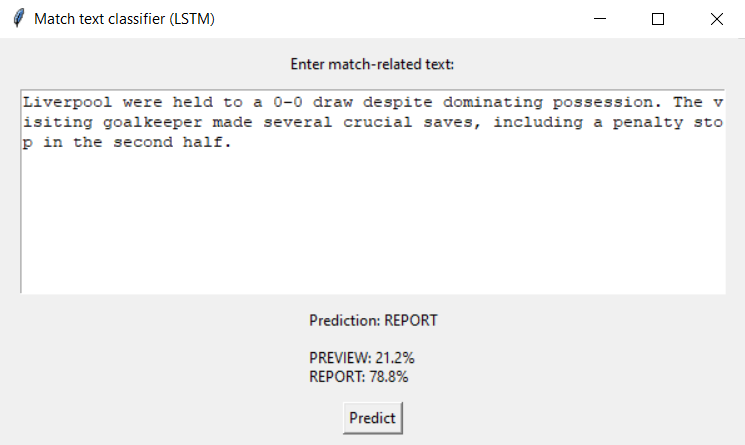
\includegraphics[width=\textwidth]{report.png}
        \caption{Klasifikacija REPORT teksta}
        \label{fig:gui_report}
    \end{minipage}\hfill
    \begin{minipage}{0.48\textwidth}
        \centering
        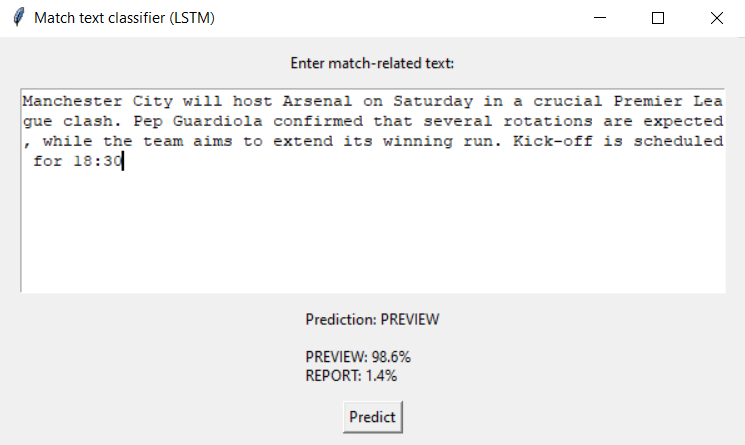
\includegraphics[width=\textwidth]{preview.png}
        \caption{Klasifikacija PREVIEW teksta}
        \label{fig:gui_preview}
    \end{minipage}
\end{figure}

Na fotografijama iznad vidimo da model s visokom sigurnosti razlikuje
najave utakmica od izvještaja nakon utakmica.

\newpage

\section{Provjera ispravnosti obrade teksta}
Budući da ispravnost obrade teksta izravno utječe na ponašanje modela, osnovne funkcije
za tokenizaciju provjerene su automatskim testovima. Za provjeru očekivanog ponašanja
funkcija \texttt{tokenize}, \texttt{make\_tokenizer} i \texttt{batch\_tokenize} koristili
smo \texttt{doctest}, čime smo testirali različite primjere ulaznog teksta.

Ukupno je izvršeno sedam doctest testova i svi su prošli. Dodatno su implementirani
\texttt{unittest} testovi za osnovne slučajeve tokenizacije, koji su također prošli. Time smo osigurali da priprema teksta daje konzistentne rezultate prije nego
što se podaci koriste u treniranju modela.


\newpage

\section{Zaključak}
U ovom radu implementiran je program za klasifikaciju sportskih tekstova, koji
obuhvaća sve ključne korake NLP pipelinea, obradu teksta, treniranje i evaluaciju
neuronskog modela. U projektu su dva pristupa, LSTM neuronski model koji koristi
sekvencijalnu obradu teksta i jednostavni baseline model temeljen
na TF--IDF reprezentaciji i logističkoj regresiji.

Rezultati pokazuju da LSTM model ima vrlo dobre performanse na skupu za testiranje
(Accuracy 0.8929, $F1_{\mathrm{macro}} = 0.8303$), pri čemu se jasno vidi razlika u
ponašanju modela po klasama. Dok su tekstovi klase \texttt{PREVIEW} uglavnom točno
klasificirani, klasa \texttt{REPORT} pokazala se problematičnijom, što se može pripisati
manjem broju dostupnih uzoraka. Upravo iz tog razloga makro F1 mjera pokazala se
prikladnijom od same točnosti za procjenu kvalitete modela.

Tijekom rada pokazali smo da ispravna priprema podataka, osobito izgradnja vokabulara, ima važan utjecaj na stabilnost i interpretaciju
rezultata. Također iz oscilacija validacijskog $F1_{\mathrm{macro}}$ vidimo osjetljivost
modela na veličinu validacijskog skupa, što je očekivana posljedica ograničene količine podataka.

Moguća buduća poboljšanja su detaljnija analiza pogrešaka (npr. kroz confusion
matrix i analizu pogrešno klasificiranih tekstova), kao i sustavnije podešavanje
hiperparametara neuronskog modela. Dodatno, zanimljiv smjer daljnjeg rada bila bi
usporedba baseline i neuronskog modela na većem i uravnoteženom skupu podataka kako
bi se jasnije procijenile prednosti sekvencijalnih modela u ovom tipu zadatka.


\newpage

\begin{thebibliography}{9}
\bibitem{jurafsky}
D. Jurafsky, J. H. Martin,
\textit{Speech and Language Processing}.

\bibitem{pytorch}
PyTorch Documentation, \url{https://pytorch.org/docs/stable/index.html}

\bibitem{sklearn}
scikit-learn Documentation, \url{https://scikit-learn.org/stable/}
\end{thebibliography}

\end{document}
